\batchmode
\documentclass[twoside]{book}

% Packages required by doxygen
\usepackage{fixltx2e}
\usepackage{calc}
\usepackage{doxygen}
\usepackage[export]{adjustbox} % also loads graphicx
\usepackage{graphicx}
\usepackage[utf8]{inputenc}
\usepackage{makeidx}
\usepackage{multicol}
\usepackage{multirow}
\PassOptionsToPackage{warn}{textcomp}
\usepackage{textcomp}
\usepackage[nointegrals]{wasysym}
\usepackage[table]{xcolor}

% Font selection
\usepackage[T1]{fontenc}
\usepackage[scaled=.90]{helvet}
\usepackage{courier}
\usepackage{amssymb}
\usepackage{sectsty}
\renewcommand{\familydefault}{\sfdefault}
\allsectionsfont{%
  \fontseries{bc}\selectfont%
  \color{darkgray}%
}
\renewcommand{\DoxyLabelFont}{%
  \fontseries{bc}\selectfont%
  \color{darkgray}%
}
\newcommand{\+}{\discretionary{\mbox{\scriptsize$\hookleftarrow$}}{}{}}

% Page & text layout
\usepackage{geometry}
\geometry{%
  a4paper,%
  top=2.5cm,%
  bottom=2.5cm,%
  left=2.5cm,%
  right=2.5cm%
}
\tolerance=750
\hfuzz=15pt
\hbadness=750
\setlength{\emergencystretch}{15pt}
\setlength{\parindent}{0cm}
\setlength{\parskip}{3ex plus 2ex minus 2ex}
\makeatletter
\renewcommand{\paragraph}{%
  \@startsection{paragraph}{4}{0ex}{-1.0ex}{1.0ex}{%
    \normalfont\normalsize\bfseries\SS@parafont%
  }%
}
\renewcommand{\subparagraph}{%
  \@startsection{subparagraph}{5}{0ex}{-1.0ex}{1.0ex}{%
    \normalfont\normalsize\bfseries\SS@subparafont%
  }%
}
\makeatother

% Headers & footers
\usepackage{fancyhdr}
\pagestyle{fancyplain}
\fancyhead[LE]{\fancyplain{}{\bfseries\thepage}}
\fancyhead[CE]{\fancyplain{}{}}
\fancyhead[RE]{\fancyplain{}{\bfseries\leftmark}}
\fancyhead[LO]{\fancyplain{}{\bfseries\rightmark}}
\fancyhead[CO]{\fancyplain{}{}}
\fancyhead[RO]{\fancyplain{}{\bfseries\thepage}}
\fancyfoot[LE]{\fancyplain{}{}}
\fancyfoot[CE]{\fancyplain{}{}}
\fancyfoot[RE]{\fancyplain{}{\bfseries\scriptsize Generated by Doxygen }}
\fancyfoot[LO]{\fancyplain{}{\bfseries\scriptsize Generated by Doxygen }}
\fancyfoot[CO]{\fancyplain{}{}}
\fancyfoot[RO]{\fancyplain{}{}}
\renewcommand{\footrulewidth}{0.4pt}
\renewcommand{\chaptermark}[1]{%
  \markboth{#1}{}%
}
\renewcommand{\sectionmark}[1]{%
  \markright{\thesection\ #1}%
}

% Indices & bibliography
\usepackage{natbib}
\usepackage[titles]{tocloft}
\setcounter{tocdepth}{3}
\setcounter{secnumdepth}{5}
\makeindex

% Hyperlinks (required, but should be loaded last)
\usepackage{ifpdf}
\ifpdf
  \usepackage[pdftex,pagebackref=true]{hyperref}
\else
  \usepackage[ps2pdf,pagebackref=true]{hyperref}
\fi
\hypersetup{%
  colorlinks=true,%
  linkcolor=blue,%
  citecolor=blue,%
  unicode%
}

% Custom commands
\newcommand{\clearemptydoublepage}{%
  \newpage{\pagestyle{empty}\cleardoublepage}%
}

\usepackage{caption}
\captionsetup{labelsep=space,justification=centering,font={bf},singlelinecheck=off,skip=4pt,position=top}

%===== C O N T E N T S =====

\begin{document}

% Titlepage & ToC
\hypersetup{pageanchor=false,
             bookmarksnumbered=true,
             pdfencoding=unicode
            }
\pagenumbering{alph}
\pagenumbering{arabic}
\hypersetup{pageanchor=true}

%--- Begin generated contents ---
\chapter{Unstructured 2D Delaunay mesh generation with xfig and Triangle}
\label{index}\hypertarget{index}{}\hypertarget{index_q}{}\section{A few quick questions...}\label{index_q}
Since {\ttfamily oomph-\/lib} is developed as open-\/source software, any evidence that the code is being downloaded and used is very helpful for us as it helps to justify our continued work on this project.

We would therefore be extremely grateful if you could provide the information requested in the form below. Pressing the \char`\"{}submit\char`\"{} button will get you to the actual download page.

{\bfseries Note\+:} 
\begin{DoxyItemize}
\item All information will be treated as confidential. 
\item If you provide your email address and check the appropriate box we will add you to our mailing list to inform you of upgrades and bug fixes to the code. Rest assured that the mailing list is {\bfseries very low volume} -- we have better things to do than to bombard you with email. 
\item If you still feel reluctant to provide any of the information requested, feel free to enter some dummy input. The form will check that {\bfseries some} information has been entered but entering your name as \char`\"{}\+Joe Cool\char`\"{} is perfectly acceptable -- this is to discourage people from not providing the information simply because they are too lazy to type... 
\end{DoxyItemize}



 







 

 \hypertarget{index_pdf}{}\section{P\+D\+F file}\label{index_pdf}
A \href{../latex/refman.pdf}{\tt pdf version} of this document is available. \end{document}

\chapter{Namespace Index}
\section{Namespace List}
Here is a list of all namespaces with brief descriptions\+:\begin{DoxyCompactList}
\item\contentsline{section}{\hyperlink{namespaceGlobal__Physical__Variables}{Global\+\_\+\+Physical\+\_\+\+Variables} \\*Global variables that represent physical properties }{\pageref{namespaceGlobal__Physical__Variables}}{}
\item\contentsline{section}{\hyperlink{namespaceoomph}{oomph} }{\pageref{namespaceoomph}}{}
\item\contentsline{section}{\hyperlink{namespacePhysical__Variables}{Physical\+\_\+\+Variables} \\*Namespace for the solution of 2D linear shell equation }{\pageref{namespacePhysical__Variables}}{}
\end{DoxyCompactList}

\chapter{Hierarchical Index}
\section{Class Hierarchy}
This inheritance list is sorted roughly, but not completely, alphabetically\+:\begin{DoxyCompactList}
\item Problem\begin{DoxyCompactList}
\item \contentsline{section}{Unstructured\+Solid\+Problem$<$ E\+L\+E\+M\+E\+NT $>$}{\pageref{classUnstructuredSolidProblem}}{}
\end{DoxyCompactList}
\end{DoxyCompactList}

\chapter{Class Index}
\section{Class List}
Here are the classes, structs, unions and interfaces with brief descriptions\+:\begin{DoxyCompactList}
\item\contentsline{section}{\hyperlink{classPMLProblem}{P\+M\+L\+Problem$<$ E\+L\+E\+M\+E\+N\+T $>$} }{\pageref{classPMLProblem}}{}
\item\contentsline{section}{\hyperlink{classGlobalParameters_1_1TestPMLMapping}{Global\+Parameters\+::\+Test\+P\+M\+L\+Mapping} }{\pageref{classGlobalParameters_1_1TestPMLMapping}}{}
\end{DoxyCompactList}

\chapter{File Index}
\section{File List}
Here is a list of all files with brief descriptions\+:\begin{DoxyCompactList}
\item\contentsline{section}{\hyperlink{jeffery__orbit_8cc}{jeffery\+\_\+orbit.\+cc} }{\pageref{jeffery__orbit_8cc}}{}
\item\contentsline{section}{\hyperlink{jeffery__orbit_8txt__doxygenified_8h}{jeffery\+\_\+orbit.\+txt\+\_\+doxygenified.\+h} }{\pageref{jeffery__orbit_8txt__doxygenified_8h}}{}
\item\contentsline{section}{\hyperlink{my__taylor__hood__elements_8h}{my\+\_\+taylor\+\_\+hood\+\_\+elements.\+h} }{\pageref{my__taylor__hood__elements_8h}}{}
\end{DoxyCompactList}

\chapter{Namespace Documentation}
\hypertarget{namespaceGlobal__Physical__Variables}{}\section{Global\+\_\+\+Physical\+\_\+\+Variables Namespace Reference}
\label{namespaceGlobal__Physical__Variables}\index{Global\+\_\+\+Physical\+\_\+\+Variables@{Global\+\_\+\+Physical\+\_\+\+Variables}}


Namespace for physical parameters.  


\subsection*{Functions}
\begin{DoxyCompactItemize}
\item 
Vector$<$ double $>$ \hyperlink{namespaceGlobal__Physical__Variables_afae321364975eb56688ad13abc8ed6b7}{Gravity} (2)
\begin{DoxyCompactList}\small\item\em Gravity vector. \end{DoxyCompactList}\item 
void \hyperlink{namespaceGlobal__Physical__Variables_a87da705b8a46bed337cf5dbdd788b87b}{body\+\_\+force} (const double \&time, const Vector$<$ double $>$ \&x, Vector$<$ double $>$ \&result)
\begin{DoxyCompactList}\small\item\em Functional body force. \end{DoxyCompactList}\item 
void \hyperlink{namespaceGlobal__Physical__Variables_a9780d615ae07c4e00a436ab2973b54e6}{zero\+\_\+body\+\_\+force} (const double \&time, const Vector$<$ double $>$ \&x, Vector$<$ double $>$ \&result)
\begin{DoxyCompactList}\small\item\em Zero functional body force. \end{DoxyCompactList}\end{DoxyCompactItemize}
\subsection*{Variables}
\begin{DoxyCompactItemize}
\item 
double \hyperlink{namespaceGlobal__Physical__Variables_ab814e627d2eb5bc50318879d19ab16b9}{Re} =100
\begin{DoxyCompactList}\small\item\em Reynolds number. \end{DoxyCompactList}\item 
double \hyperlink{namespaceGlobal__Physical__Variables_ab1a845a672b4d74b304639a976dc65c6}{Re\+\_\+inv\+Fr} =100
\begin{DoxyCompactList}\small\item\em Reynolds/\+Froude number. \end{DoxyCompactList}\end{DoxyCompactItemize}


\subsection{Detailed Description}
Namespace for physical parameters. 

\subsection{Function Documentation}
\mbox{\Hypertarget{namespaceGlobal__Physical__Variables_a87da705b8a46bed337cf5dbdd788b87b}\label{namespaceGlobal__Physical__Variables_a87da705b8a46bed337cf5dbdd788b87b}} 
\index{Global\+\_\+\+Physical\+\_\+\+Variables@{Global\+\_\+\+Physical\+\_\+\+Variables}!body\+\_\+force@{body\+\_\+force}}
\index{body\+\_\+force@{body\+\_\+force}!Global\+\_\+\+Physical\+\_\+\+Variables@{Global\+\_\+\+Physical\+\_\+\+Variables}}
\subsubsection{\texorpdfstring{body\+\_\+force()}{body\_force()}}
{\footnotesize\ttfamily void Global\+\_\+\+Physical\+\_\+\+Variables\+::body\+\_\+force (\begin{DoxyParamCaption}\item[{const double \&}]{time,  }\item[{const Vector$<$ double $>$ \&}]{x,  }\item[{Vector$<$ double $>$ \&}]{result }\end{DoxyParamCaption})}



Functional body force. 



Definition at line 62 of file circular\+\_\+driven\+\_\+cavity.\+cc.



References Re\+\_\+inv\+Fr.



Referenced by main().

\mbox{\Hypertarget{namespaceGlobal__Physical__Variables_afae321364975eb56688ad13abc8ed6b7}\label{namespaceGlobal__Physical__Variables_afae321364975eb56688ad13abc8ed6b7}} 
\index{Global\+\_\+\+Physical\+\_\+\+Variables@{Global\+\_\+\+Physical\+\_\+\+Variables}!Gravity@{Gravity}}
\index{Gravity@{Gravity}!Global\+\_\+\+Physical\+\_\+\+Variables@{Global\+\_\+\+Physical\+\_\+\+Variables}}
\subsubsection{\texorpdfstring{Gravity()}{Gravity()}}
{\footnotesize\ttfamily Vector$<$double$>$ Global\+\_\+\+Physical\+\_\+\+Variables\+::\+Gravity (\begin{DoxyParamCaption}\item[{2}]{ }\end{DoxyParamCaption})}



Gravity vector. 



Referenced by main(), and Quarter\+Circle\+Driven\+Cavity\+Problem$<$ E\+L\+E\+M\+E\+N\+T $>$\+::\+Quarter\+Circle\+Driven\+Cavity\+Problem().

\mbox{\Hypertarget{namespaceGlobal__Physical__Variables_a9780d615ae07c4e00a436ab2973b54e6}\label{namespaceGlobal__Physical__Variables_a9780d615ae07c4e00a436ab2973b54e6}} 
\index{Global\+\_\+\+Physical\+\_\+\+Variables@{Global\+\_\+\+Physical\+\_\+\+Variables}!zero\+\_\+body\+\_\+force@{zero\+\_\+body\+\_\+force}}
\index{zero\+\_\+body\+\_\+force@{zero\+\_\+body\+\_\+force}!Global\+\_\+\+Physical\+\_\+\+Variables@{Global\+\_\+\+Physical\+\_\+\+Variables}}
\subsubsection{\texorpdfstring{zero\+\_\+body\+\_\+force()}{zero\_body\_force()}}
{\footnotesize\ttfamily void Global\+\_\+\+Physical\+\_\+\+Variables\+::zero\+\_\+body\+\_\+force (\begin{DoxyParamCaption}\item[{const double \&}]{time,  }\item[{const Vector$<$ double $>$ \&}]{x,  }\item[{Vector$<$ double $>$ \&}]{result }\end{DoxyParamCaption})}



Zero functional body force. 



Definition at line 70 of file circular\+\_\+driven\+\_\+cavity.\+cc.



Referenced by main().



\subsection{Variable Documentation}
\mbox{\Hypertarget{namespaceGlobal__Physical__Variables_ab814e627d2eb5bc50318879d19ab16b9}\label{namespaceGlobal__Physical__Variables_ab814e627d2eb5bc50318879d19ab16b9}} 
\index{Global\+\_\+\+Physical\+\_\+\+Variables@{Global\+\_\+\+Physical\+\_\+\+Variables}!Re@{Re}}
\index{Re@{Re}!Global\+\_\+\+Physical\+\_\+\+Variables@{Global\+\_\+\+Physical\+\_\+\+Variables}}
\subsubsection{\texorpdfstring{Re}{Re}}
{\footnotesize\ttfamily double Global\+\_\+\+Physical\+\_\+\+Variables\+::\+Re =100}



Reynolds number. 



Definition at line 53 of file circular\+\_\+driven\+\_\+cavity.\+cc.



Referenced by Quarter\+Circle\+Driven\+Cavity\+Problem$<$ E\+L\+E\+M\+E\+N\+T $>$\+::\+Quarter\+Circle\+Driven\+Cavity\+Problem().

\mbox{\Hypertarget{namespaceGlobal__Physical__Variables_ab1a845a672b4d74b304639a976dc65c6}\label{namespaceGlobal__Physical__Variables_ab1a845a672b4d74b304639a976dc65c6}} 
\index{Global\+\_\+\+Physical\+\_\+\+Variables@{Global\+\_\+\+Physical\+\_\+\+Variables}!Re\+\_\+inv\+Fr@{Re\+\_\+inv\+Fr}}
\index{Re\+\_\+inv\+Fr@{Re\+\_\+inv\+Fr}!Global\+\_\+\+Physical\+\_\+\+Variables@{Global\+\_\+\+Physical\+\_\+\+Variables}}
\subsubsection{\texorpdfstring{Re\+\_\+inv\+Fr}{Re\_invFr}}
{\footnotesize\ttfamily double Global\+\_\+\+Physical\+\_\+\+Variables\+::\+Re\+\_\+inv\+Fr =100}



Reynolds/\+Froude number. 



Definition at line 56 of file circular\+\_\+driven\+\_\+cavity.\+cc.



Referenced by body\+\_\+force(), and Quarter\+Circle\+Driven\+Cavity\+Problem$<$ E\+L\+E\+M\+E\+N\+T $>$\+::\+Quarter\+Circle\+Driven\+Cavity\+Problem().


\hypertarget{namespaceTanhSolnForPoisson}{}\section{Tanh\+Soln\+For\+Poisson Namespace Reference}
\label{namespaceTanhSolnForPoisson}\index{Tanh\+Soln\+For\+Poisson@{Tanh\+Soln\+For\+Poisson}}


Namespace for exact solution for Poisson equation with sharp step.  


\subsection*{Functions}
\begin{DoxyCompactItemize}
\item 
void \hyperlink{namespaceTanhSolnForPoisson_af7896e9c18ce6438c73ae2a875e8b7de}{get\+\_\+exact\+\_\+u} (const Vector$<$ double $>$ \&x, Vector$<$ double $>$ \&u)
\begin{DoxyCompactList}\small\item\em Exact solution as a Vector. \end{DoxyCompactList}\item 
void \hyperlink{namespaceTanhSolnForPoisson_af197decab980d38d2037032780723984}{get\+\_\+exact\+\_\+u} (const Vector$<$ double $>$ \&x, double \&u)
\begin{DoxyCompactList}\small\item\em Exact solution as a scalar. \end{DoxyCompactList}\item 
void \hyperlink{namespaceTanhSolnForPoisson_ae1b9d6789ff301e3d63a4e292213036c}{get\+\_\+source} (const Vector$<$ double $>$ \&x, double \&source)
\begin{DoxyCompactList}\small\item\em Source function to make it an exact solution. \end{DoxyCompactList}\end{DoxyCompactItemize}
\subsection*{Variables}
\begin{DoxyCompactItemize}
\item 
double \hyperlink{namespaceTanhSolnForPoisson_ae676ccd186d5df119cce811596d949c1}{Alpha}
\begin{DoxyCompactList}\small\item\em Parameter for steepness of step. \end{DoxyCompactList}\item 
double \hyperlink{namespaceTanhSolnForPoisson_ae07364a1d73b28e5e250bda6c8954f01}{Beta}
\begin{DoxyCompactList}\small\item\em Parameter for angle of step. \end{DoxyCompactList}\end{DoxyCompactItemize}


\subsection{Detailed Description}
Namespace for exact solution for Poisson equation with sharp step. 

\subsection{Function Documentation}
\mbox{\Hypertarget{namespaceTanhSolnForPoisson_af7896e9c18ce6438c73ae2a875e8b7de}\label{namespaceTanhSolnForPoisson_af7896e9c18ce6438c73ae2a875e8b7de}} 
\index{Tanh\+Soln\+For\+Poisson@{Tanh\+Soln\+For\+Poisson}!get\+\_\+exact\+\_\+u@{get\+\_\+exact\+\_\+u}}
\index{get\+\_\+exact\+\_\+u@{get\+\_\+exact\+\_\+u}!Tanh\+Soln\+For\+Poisson@{Tanh\+Soln\+For\+Poisson}}
\subsubsection{\texorpdfstring{get\+\_\+exact\+\_\+u()}{get\_exact\_u()}\hspace{0.1cm}{\footnotesize\ttfamily [1/2]}}
{\footnotesize\ttfamily void Tanh\+Soln\+For\+Poisson\+::get\+\_\+exact\+\_\+u (\begin{DoxyParamCaption}\item[{const Vector$<$ double $>$ \&}]{x,  }\item[{Vector$<$ double $>$ \&}]{u }\end{DoxyParamCaption})}



Exact solution as a Vector. 



Definition at line 61 of file mesh\+\_\+from\+\_\+triangle\+\_\+poisson.\+cc.



Referenced by Poisson\+Problem$<$ E\+L\+E\+M\+E\+N\+T $>$\+::actions\+\_\+before\+\_\+newton\+\_\+solve(), and Poisson\+Problem$<$ E\+L\+E\+M\+E\+N\+T $>$\+::doc\+\_\+solution().

\mbox{\Hypertarget{namespaceTanhSolnForPoisson_af197decab980d38d2037032780723984}\label{namespaceTanhSolnForPoisson_af197decab980d38d2037032780723984}} 
\index{Tanh\+Soln\+For\+Poisson@{Tanh\+Soln\+For\+Poisson}!get\+\_\+exact\+\_\+u@{get\+\_\+exact\+\_\+u}}
\index{get\+\_\+exact\+\_\+u@{get\+\_\+exact\+\_\+u}!Tanh\+Soln\+For\+Poisson@{Tanh\+Soln\+For\+Poisson}}
\subsubsection{\texorpdfstring{get\+\_\+exact\+\_\+u()}{get\_exact\_u()}\hspace{0.1cm}{\footnotesize\ttfamily [2/2]}}
{\footnotesize\ttfamily void Tanh\+Soln\+For\+Poisson\+::get\+\_\+exact\+\_\+u (\begin{DoxyParamCaption}\item[{const Vector$<$ double $>$ \&}]{x,  }\item[{double \&}]{u }\end{DoxyParamCaption})}



Exact solution as a scalar. 



Definition at line 68 of file mesh\+\_\+from\+\_\+triangle\+\_\+poisson.\+cc.

\mbox{\Hypertarget{namespaceTanhSolnForPoisson_ae1b9d6789ff301e3d63a4e292213036c}\label{namespaceTanhSolnForPoisson_ae1b9d6789ff301e3d63a4e292213036c}} 
\index{Tanh\+Soln\+For\+Poisson@{Tanh\+Soln\+For\+Poisson}!get\+\_\+source@{get\+\_\+source}}
\index{get\+\_\+source@{get\+\_\+source}!Tanh\+Soln\+For\+Poisson@{Tanh\+Soln\+For\+Poisson}}
\subsubsection{\texorpdfstring{get\+\_\+source()}{get\_source()}}
{\footnotesize\ttfamily void Tanh\+Soln\+For\+Poisson\+::get\+\_\+source (\begin{DoxyParamCaption}\item[{const Vector$<$ double $>$ \&}]{x,  }\item[{double \&}]{source }\end{DoxyParamCaption})}



Source function to make it an exact solution. 



Definition at line 75 of file mesh\+\_\+from\+\_\+triangle\+\_\+poisson.\+cc.



Referenced by main().



\subsection{Variable Documentation}
\mbox{\Hypertarget{namespaceTanhSolnForPoisson_ae676ccd186d5df119cce811596d949c1}\label{namespaceTanhSolnForPoisson_ae676ccd186d5df119cce811596d949c1}} 
\index{Tanh\+Soln\+For\+Poisson@{Tanh\+Soln\+For\+Poisson}!Alpha@{Alpha}}
\index{Alpha@{Alpha}!Tanh\+Soln\+For\+Poisson@{Tanh\+Soln\+For\+Poisson}}
\subsubsection{\texorpdfstring{Alpha}{Alpha}}
{\footnotesize\ttfamily double Tanh\+Soln\+For\+Poisson\+::\+Alpha}



Parameter for steepness of step. 



Definition at line 54 of file mesh\+\_\+from\+\_\+triangle\+\_\+poisson.\+cc.



Referenced by Poisson\+Problem$<$ E\+L\+E\+M\+E\+N\+T $>$\+::\+Poisson\+Problem().

\mbox{\Hypertarget{namespaceTanhSolnForPoisson_ae07364a1d73b28e5e250bda6c8954f01}\label{namespaceTanhSolnForPoisson_ae07364a1d73b28e5e250bda6c8954f01}} 
\index{Tanh\+Soln\+For\+Poisson@{Tanh\+Soln\+For\+Poisson}!Beta@{Beta}}
\index{Beta@{Beta}!Tanh\+Soln\+For\+Poisson@{Tanh\+Soln\+For\+Poisson}}
\subsubsection{\texorpdfstring{Beta}{Beta}}
{\footnotesize\ttfamily double Tanh\+Soln\+For\+Poisson\+::\+Beta}



Parameter for angle of step. 



Definition at line 57 of file mesh\+\_\+from\+\_\+triangle\+\_\+poisson.\+cc.



Referenced by Poisson\+Problem$<$ E\+L\+E\+M\+E\+N\+T $>$\+::\+Poisson\+Problem().


\chapter{Class Documentation}
\hypertarget{classFlowPastBoxProblem}{}\section{Flow\+Past\+Box\+Problem$<$ E\+L\+E\+M\+E\+NT $>$ Class Template Reference}
\label{classFlowPastBoxProblem}\index{Flow\+Past\+Box\+Problem$<$ E\+L\+E\+M\+E\+N\+T $>$@{Flow\+Past\+Box\+Problem$<$ E\+L\+E\+M\+E\+N\+T $>$}}


Flow past a box in a channel.  


Inheritance diagram for Flow\+Past\+Box\+Problem$<$ E\+L\+E\+M\+E\+NT $>$\+:\begin{figure}[H]
\begin{center}
\leavevmode
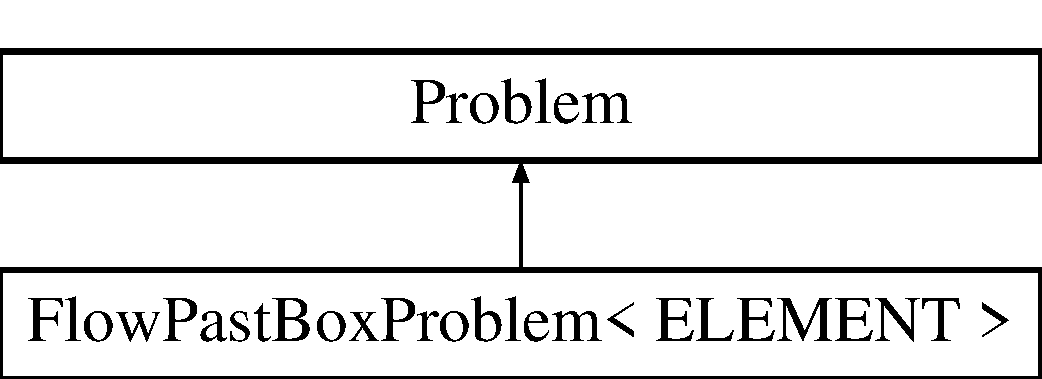
\includegraphics[height=2.000000cm]{classFlowPastBoxProblem}
\end{center}
\end{figure}
\subsection*{Public Member Functions}
\begin{DoxyCompactItemize}
\item 
\hyperlink{classFlowPastBoxProblem_a6b674c1028abcd6e54c50d939d25a00e}{Flow\+Past\+Box\+Problem} (const string \&node\+\_\+file\+\_\+name, const string \&element\+\_\+file\+\_\+name, const string \&poly\+\_\+file\+\_\+name)
\begin{DoxyCompactList}\small\item\em Constructor\+: Pass filenames for mesh. \end{DoxyCompactList}\item 
\hyperlink{classFlowPastBoxProblem_a48bb150799924e3d0ab42a610babefbd}{$\sim$\+Flow\+Past\+Box\+Problem} ()
\begin{DoxyCompactList}\small\item\em Destructor (empty) \end{DoxyCompactList}\item 
void \hyperlink{classFlowPastBoxProblem_a5d226368814cfbf84f274a63b3c0b20c}{actions\+\_\+after\+\_\+newton\+\_\+solve} ()
\begin{DoxyCompactList}\small\item\em Update the after solve (empty) \end{DoxyCompactList}\item 
void \hyperlink{classFlowPastBoxProblem_a602772b5e37d5bd426d64e46cc3f59ea}{actions\+\_\+before\+\_\+newton\+\_\+solve} ()
\begin{DoxyCompactList}\small\item\em Update the problem specs before solve. Re-\/set velocity boundary conditions just to be on the safe side... \end{DoxyCompactList}\item 
void \hyperlink{classFlowPastBoxProblem_a726b784a8c4c4cbfff1a870ed9d01d28}{actions\+\_\+after\+\_\+adapt} ()
\item 
\hyperlink{classoomph_1_1RefineableTriangleMesh}{Refineable\+Triangle\+Mesh}$<$ E\+L\+E\+M\+E\+NT $>$ $\ast$ \hyperlink{classFlowPastBoxProblem_a61a6212a46def12d33d68453489f4379}{mesh\+\_\+pt} ()
\begin{DoxyCompactList}\small\item\em Access function for the specific mesh. \end{DoxyCompactList}\item 
\hyperlink{classoomph_1_1TriangleMesh}{Triangle\+Mesh}$<$ E\+L\+E\+M\+E\+NT $>$ $\ast$ \hyperlink{classFlowPastBoxProblem_a3efbee75a2cc6ca9d6ffd4ec0a3a2c52}{mesh\+\_\+pt} ()
\begin{DoxyCompactList}\small\item\em Access function for the specific mesh. \end{DoxyCompactList}\item 
void \hyperlink{classFlowPastBoxProblem_a7e2f3692ab8f492c6d5e967953c4a4ea}{doc\+\_\+solution} (Doc\+Info \&doc\+\_\+info)
\begin{DoxyCompactList}\small\item\em Doc the solution. \end{DoxyCompactList}\end{DoxyCompactItemize}
\subsection*{Private Attributes}
\begin{DoxyCompactItemize}
\item 
\hyperlink{classoomph_1_1RefineableTriangleMesh}{Refineable\+Triangle\+Mesh}$<$ E\+L\+E\+M\+E\+NT $>$ $\ast$ \hyperlink{classFlowPastBoxProblem_a5ffdeb61acb20f9c154fafad3c0196e8}{Bulk\+\_\+mesh\+\_\+pt}
\begin{DoxyCompactList}\small\item\em Pointer to the bulk mesh. \end{DoxyCompactList}\item 
Z2\+Error\+Estimator $\ast$ \hyperlink{classFlowPastBoxProblem_a44b20a7eb85ce8a902da6c6275f45278}{error\+\_\+estimator\+\_\+pt}
\begin{DoxyCompactList}\small\item\em Error estimator. \end{DoxyCompactList}\end{DoxyCompactItemize}


\subsection{Detailed Description}
\subsubsection*{template$<$class E\+L\+E\+M\+E\+NT$>$\newline
class Flow\+Past\+Box\+Problem$<$ E\+L\+E\+M\+E\+N\+T $>$}

Flow past a box in a channel. 

Definition at line 66 of file mesh\+\_\+from\+\_\+triangle\+\_\+navier\+\_\+stokes.\+cc.



\subsection{Constructor \& Destructor Documentation}
\mbox{\Hypertarget{classFlowPastBoxProblem_a6b674c1028abcd6e54c50d939d25a00e}\label{classFlowPastBoxProblem_a6b674c1028abcd6e54c50d939d25a00e}} 
\index{Flow\+Past\+Box\+Problem@{Flow\+Past\+Box\+Problem}!Flow\+Past\+Box\+Problem@{Flow\+Past\+Box\+Problem}}
\index{Flow\+Past\+Box\+Problem@{Flow\+Past\+Box\+Problem}!Flow\+Past\+Box\+Problem@{Flow\+Past\+Box\+Problem}}
\subsubsection{\texorpdfstring{Flow\+Past\+Box\+Problem()}{FlowPastBoxProblem()}}
{\footnotesize\ttfamily template$<$class E\+L\+E\+M\+E\+NT $>$ \\
\hyperlink{classFlowPastBoxProblem}{Flow\+Past\+Box\+Problem}$<$ E\+L\+E\+M\+E\+NT $>$\+::\hyperlink{classFlowPastBoxProblem}{Flow\+Past\+Box\+Problem} (\begin{DoxyParamCaption}\item[{const string \&}]{node\+\_\+file\+\_\+name,  }\item[{const string \&}]{element\+\_\+file\+\_\+name,  }\item[{const string \&}]{poly\+\_\+file\+\_\+name }\end{DoxyParamCaption})}



Constructor\+: Pass filenames for mesh. 

Constructor for Flow\+Past\+Box problem. Pass filenames for mesh. 

Definition at line 168 of file mesh\+\_\+from\+\_\+triangle\+\_\+navier\+\_\+stokes.\+cc.



References Global\+\_\+\+Physical\+\_\+\+Variables\+::\+Re.

\mbox{\Hypertarget{classFlowPastBoxProblem_a48bb150799924e3d0ab42a610babefbd}\label{classFlowPastBoxProblem_a48bb150799924e3d0ab42a610babefbd}} 
\index{Flow\+Past\+Box\+Problem@{Flow\+Past\+Box\+Problem}!````~Flow\+Past\+Box\+Problem@{$\sim$\+Flow\+Past\+Box\+Problem}}
\index{````~Flow\+Past\+Box\+Problem@{$\sim$\+Flow\+Past\+Box\+Problem}!Flow\+Past\+Box\+Problem@{Flow\+Past\+Box\+Problem}}
\subsubsection{\texorpdfstring{$\sim$\+Flow\+Past\+Box\+Problem()}{~FlowPastBoxProblem()}}
{\footnotesize\ttfamily template$<$class E\+L\+E\+M\+E\+NT$>$ \\
\hyperlink{classFlowPastBoxProblem}{Flow\+Past\+Box\+Problem}$<$ E\+L\+E\+M\+E\+NT $>$\+::$\sim$\hyperlink{classFlowPastBoxProblem}{Flow\+Past\+Box\+Problem} (\begin{DoxyParamCaption}{ }\end{DoxyParamCaption})\hspace{0.3cm}{\ttfamily [inline]}}



Destructor (empty) 



Definition at line 78 of file mesh\+\_\+from\+\_\+triangle\+\_\+navier\+\_\+stokes.\+cc.



\subsection{Member Function Documentation}
\mbox{\Hypertarget{classFlowPastBoxProblem_a726b784a8c4c4cbfff1a870ed9d01d28}\label{classFlowPastBoxProblem_a726b784a8c4c4cbfff1a870ed9d01d28}} 
\index{Flow\+Past\+Box\+Problem@{Flow\+Past\+Box\+Problem}!actions\+\_\+after\+\_\+adapt@{actions\+\_\+after\+\_\+adapt}}
\index{actions\+\_\+after\+\_\+adapt@{actions\+\_\+after\+\_\+adapt}!Flow\+Past\+Box\+Problem@{Flow\+Past\+Box\+Problem}}
\subsubsection{\texorpdfstring{actions\+\_\+after\+\_\+adapt()}{actions\_after\_adapt()}}
{\footnotesize\ttfamily template$<$class E\+L\+E\+M\+E\+NT $>$ \\
void \hyperlink{classFlowPastBoxProblem}{Flow\+Past\+Box\+Problem}$<$ E\+L\+E\+M\+E\+NT $>$\+::actions\+\_\+after\+\_\+adapt (\begin{DoxyParamCaption}{ }\end{DoxyParamCaption})}



Definition at line 243 of file mesh\+\_\+from\+\_\+triangle\+\_\+navier\+\_\+stokes.\+cc.



References Global\+\_\+\+Physical\+\_\+\+Variables\+::\+Re.

\mbox{\Hypertarget{classFlowPastBoxProblem_a5d226368814cfbf84f274a63b3c0b20c}\label{classFlowPastBoxProblem_a5d226368814cfbf84f274a63b3c0b20c}} 
\index{Flow\+Past\+Box\+Problem@{Flow\+Past\+Box\+Problem}!actions\+\_\+after\+\_\+newton\+\_\+solve@{actions\+\_\+after\+\_\+newton\+\_\+solve}}
\index{actions\+\_\+after\+\_\+newton\+\_\+solve@{actions\+\_\+after\+\_\+newton\+\_\+solve}!Flow\+Past\+Box\+Problem@{Flow\+Past\+Box\+Problem}}
\subsubsection{\texorpdfstring{actions\+\_\+after\+\_\+newton\+\_\+solve()}{actions\_after\_newton\_solve()}}
{\footnotesize\ttfamily template$<$class E\+L\+E\+M\+E\+NT$>$ \\
void \hyperlink{classFlowPastBoxProblem}{Flow\+Past\+Box\+Problem}$<$ E\+L\+E\+M\+E\+NT $>$\+::actions\+\_\+after\+\_\+newton\+\_\+solve (\begin{DoxyParamCaption}{ }\end{DoxyParamCaption})\hspace{0.3cm}{\ttfamily [inline]}}



Update the after solve (empty) 



Definition at line 81 of file mesh\+\_\+from\+\_\+triangle\+\_\+navier\+\_\+stokes.\+cc.

\mbox{\Hypertarget{classFlowPastBoxProblem_a602772b5e37d5bd426d64e46cc3f59ea}\label{classFlowPastBoxProblem_a602772b5e37d5bd426d64e46cc3f59ea}} 
\index{Flow\+Past\+Box\+Problem@{Flow\+Past\+Box\+Problem}!actions\+\_\+before\+\_\+newton\+\_\+solve@{actions\+\_\+before\+\_\+newton\+\_\+solve}}
\index{actions\+\_\+before\+\_\+newton\+\_\+solve@{actions\+\_\+before\+\_\+newton\+\_\+solve}!Flow\+Past\+Box\+Problem@{Flow\+Past\+Box\+Problem}}
\subsubsection{\texorpdfstring{actions\+\_\+before\+\_\+newton\+\_\+solve()}{actions\_before\_newton\_solve()}}
{\footnotesize\ttfamily template$<$class E\+L\+E\+M\+E\+NT$>$ \\
void \hyperlink{classFlowPastBoxProblem}{Flow\+Past\+Box\+Problem}$<$ E\+L\+E\+M\+E\+NT $>$\+::actions\+\_\+before\+\_\+newton\+\_\+solve (\begin{DoxyParamCaption}{ }\end{DoxyParamCaption})\hspace{0.3cm}{\ttfamily [inline]}}



Update the problem specs before solve. Re-\/set velocity boundary conditions just to be on the safe side... 



Definition at line 85 of file mesh\+\_\+from\+\_\+triangle\+\_\+navier\+\_\+stokes.\+cc.

\mbox{\Hypertarget{classFlowPastBoxProblem_a7e2f3692ab8f492c6d5e967953c4a4ea}\label{classFlowPastBoxProblem_a7e2f3692ab8f492c6d5e967953c4a4ea}} 
\index{Flow\+Past\+Box\+Problem@{Flow\+Past\+Box\+Problem}!doc\+\_\+solution@{doc\+\_\+solution}}
\index{doc\+\_\+solution@{doc\+\_\+solution}!Flow\+Past\+Box\+Problem@{Flow\+Past\+Box\+Problem}}
\subsubsection{\texorpdfstring{doc\+\_\+solution()}{doc\_solution()}}
{\footnotesize\ttfamily template$<$class E\+L\+E\+M\+E\+NT $>$ \\
void \hyperlink{classFlowPastBoxProblem}{Flow\+Past\+Box\+Problem}$<$ E\+L\+E\+M\+E\+NT $>$\+::doc\+\_\+solution (\begin{DoxyParamCaption}\item[{Doc\+Info \&}]{doc\+\_\+info }\end{DoxyParamCaption})}



Doc the solution. 



Definition at line 297 of file mesh\+\_\+from\+\_\+triangle\+\_\+navier\+\_\+stokes.\+cc.



Referenced by main().

\mbox{\Hypertarget{classFlowPastBoxProblem_a61a6212a46def12d33d68453489f4379}\label{classFlowPastBoxProblem_a61a6212a46def12d33d68453489f4379}} 
\index{Flow\+Past\+Box\+Problem@{Flow\+Past\+Box\+Problem}!mesh\+\_\+pt@{mesh\+\_\+pt}}
\index{mesh\+\_\+pt@{mesh\+\_\+pt}!Flow\+Past\+Box\+Problem@{Flow\+Past\+Box\+Problem}}
\subsubsection{\texorpdfstring{mesh\+\_\+pt()}{mesh\_pt()}\hspace{0.1cm}{\footnotesize\ttfamily [1/2]}}
{\footnotesize\ttfamily template$<$class E\+L\+E\+M\+E\+NT$>$ \\
\hyperlink{classoomph_1_1RefineableTriangleMesh}{Refineable\+Triangle\+Mesh}$<$E\+L\+E\+M\+E\+NT$>$$\ast$ \hyperlink{classFlowPastBoxProblem}{Flow\+Past\+Box\+Problem}$<$ E\+L\+E\+M\+E\+NT $>$\+::mesh\+\_\+pt (\begin{DoxyParamCaption}{ }\end{DoxyParamCaption})\hspace{0.3cm}{\ttfamily [inline]}}



Access function for the specific mesh. 



Definition at line 136 of file mesh\+\_\+from\+\_\+triangle\+\_\+navier\+\_\+stokes.\+cc.



Referenced by main().

\mbox{\Hypertarget{classFlowPastBoxProblem_a3efbee75a2cc6ca9d6ffd4ec0a3a2c52}\label{classFlowPastBoxProblem_a3efbee75a2cc6ca9d6ffd4ec0a3a2c52}} 
\index{Flow\+Past\+Box\+Problem@{Flow\+Past\+Box\+Problem}!mesh\+\_\+pt@{mesh\+\_\+pt}}
\index{mesh\+\_\+pt@{mesh\+\_\+pt}!Flow\+Past\+Box\+Problem@{Flow\+Past\+Box\+Problem}}
\subsubsection{\texorpdfstring{mesh\+\_\+pt()}{mesh\_pt()}\hspace{0.1cm}{\footnotesize\ttfamily [2/2]}}
{\footnotesize\ttfamily template$<$class E\+L\+E\+M\+E\+NT$>$ \\
\hyperlink{classoomph_1_1TriangleMesh}{Triangle\+Mesh}$<$E\+L\+E\+M\+E\+NT$>$$\ast$ \hyperlink{classFlowPastBoxProblem}{Flow\+Past\+Box\+Problem}$<$ E\+L\+E\+M\+E\+NT $>$\+::mesh\+\_\+pt (\begin{DoxyParamCaption}{ }\end{DoxyParamCaption})\hspace{0.3cm}{\ttfamily [inline]}}



Access function for the specific mesh. 



Definition at line 142 of file mesh\+\_\+from\+\_\+triangle\+\_\+navier\+\_\+stokes.\+cc.



\subsection{Member Data Documentation}
\mbox{\Hypertarget{classFlowPastBoxProblem_a5ffdeb61acb20f9c154fafad3c0196e8}\label{classFlowPastBoxProblem_a5ffdeb61acb20f9c154fafad3c0196e8}} 
\index{Flow\+Past\+Box\+Problem@{Flow\+Past\+Box\+Problem}!Bulk\+\_\+mesh\+\_\+pt@{Bulk\+\_\+mesh\+\_\+pt}}
\index{Bulk\+\_\+mesh\+\_\+pt@{Bulk\+\_\+mesh\+\_\+pt}!Flow\+Past\+Box\+Problem@{Flow\+Past\+Box\+Problem}}
\subsubsection{\texorpdfstring{Bulk\+\_\+mesh\+\_\+pt}{Bulk\_mesh\_pt}}
{\footnotesize\ttfamily template$<$class E\+L\+E\+M\+E\+NT$>$ \\
\hyperlink{classoomph_1_1RefineableTriangleMesh}{Refineable\+Triangle\+Mesh}$<$E\+L\+E\+M\+E\+NT$>$$\ast$ \hyperlink{classFlowPastBoxProblem}{Flow\+Past\+Box\+Problem}$<$ E\+L\+E\+M\+E\+NT $>$\+::Bulk\+\_\+mesh\+\_\+pt\hspace{0.3cm}{\ttfamily [private]}}



Pointer to the bulk mesh. 



Definition at line 154 of file mesh\+\_\+from\+\_\+triangle\+\_\+navier\+\_\+stokes.\+cc.

\mbox{\Hypertarget{classFlowPastBoxProblem_a44b20a7eb85ce8a902da6c6275f45278}\label{classFlowPastBoxProblem_a44b20a7eb85ce8a902da6c6275f45278}} 
\index{Flow\+Past\+Box\+Problem@{Flow\+Past\+Box\+Problem}!error\+\_\+estimator\+\_\+pt@{error\+\_\+estimator\+\_\+pt}}
\index{error\+\_\+estimator\+\_\+pt@{error\+\_\+estimator\+\_\+pt}!Flow\+Past\+Box\+Problem@{Flow\+Past\+Box\+Problem}}
\subsubsection{\texorpdfstring{error\+\_\+estimator\+\_\+pt}{error\_estimator\_pt}}
{\footnotesize\ttfamily template$<$class E\+L\+E\+M\+E\+NT$>$ \\
Z2\+Error\+Estimator$\ast$ \hyperlink{classFlowPastBoxProblem}{Flow\+Past\+Box\+Problem}$<$ E\+L\+E\+M\+E\+NT $>$\+::error\+\_\+estimator\+\_\+pt\hspace{0.3cm}{\ttfamily [private]}}



Error estimator. 



Definition at line 157 of file mesh\+\_\+from\+\_\+triangle\+\_\+navier\+\_\+stokes.\+cc.



The documentation for this class was generated from the following file\+:\begin{DoxyCompactItemize}
\item 
\hyperlink{mesh__from__triangle__navier__stokes_8cc}{mesh\+\_\+from\+\_\+triangle\+\_\+navier\+\_\+stokes.\+cc}\end{DoxyCompactItemize}

\hypertarget{classPoissonProblem}{}\section{Poisson\+Problem$<$ E\+L\+E\+M\+E\+NT $>$ Class Template Reference}
\label{classPoissonProblem}\index{Poisson\+Problem$<$ E\+L\+E\+M\+E\+N\+T $>$@{Poisson\+Problem$<$ E\+L\+E\+M\+E\+N\+T $>$}}
Inheritance diagram for Poisson\+Problem$<$ E\+L\+E\+M\+E\+NT $>$\+:\begin{figure}[H]
\begin{center}
\leavevmode
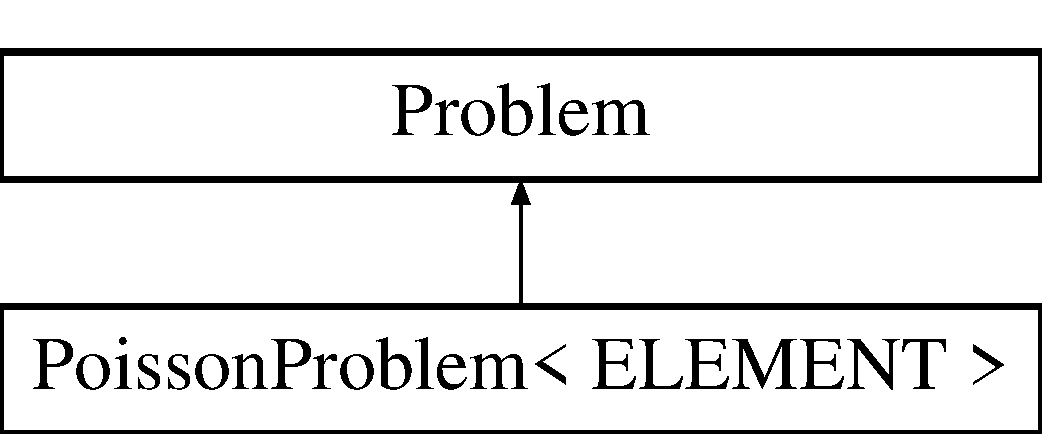
\includegraphics[height=1.944445cm]{classPoissonProblem}
\end{center}
\end{figure}
\subsection*{Public Member Functions}
\begin{DoxyCompactItemize}
\item 
\hyperlink{classPoissonProblem_a9c28346c473d246d8f61022365e742ea}{Poisson\+Problem} (Poisson\+Equations$<$ 2 $>$\+::Poisson\+Source\+Fct\+Pt source\+\_\+fct\+\_\+pt)
\begin{DoxyCompactList}\small\item\em Constructor\+: Pass pointer to source function. \end{DoxyCompactList}\item 
\hyperlink{classPoissonProblem_ac247e42d2d292200617f4b9db7ed1ab8}{$\sim$\+Poisson\+Problem} ()
\begin{DoxyCompactList}\small\item\em Destructor (empty) \end{DoxyCompactList}\item 
void \hyperlink{classPoissonProblem_a398608a5ff73b74c5a387b3f794c58df}{actions\+\_\+before\+\_\+newton\+\_\+solve} ()
\begin{DoxyCompactList}\small\item\em Update the problem specs before solve\+: Reset boundary conditions to the values from the exact solution. \end{DoxyCompactList}\item 
void \hyperlink{classPoissonProblem_a7a9478d8e1e5c7d3a886b00ab7d50bbd}{actions\+\_\+after\+\_\+newton\+\_\+solve} ()
\begin{DoxyCompactList}\small\item\em Update the problem after solve (empty) \end{DoxyCompactList}\item 
void \hyperlink{classPoissonProblem_aab6f503fa242f687bb8452527bb7688f}{doc\+\_\+solution} (Doc\+Info \&doc\+\_\+info)
\begin{DoxyCompactList}\small\item\em Doc the solution. Doc\+Info object stores flags/labels for where the output gets written to. \end{DoxyCompactList}\item 
\hyperlink{classPoissonProblem_a9c28346c473d246d8f61022365e742ea}{Poisson\+Problem} (Poisson\+Equations$<$ 2 $>$\+::Poisson\+Source\+Fct\+Pt source\+\_\+fct\+\_\+pt)
\begin{DoxyCompactList}\small\item\em Constructor\+: Pass pointer to source function. \end{DoxyCompactList}\item 
\hyperlink{classPoissonProblem_ac247e42d2d292200617f4b9db7ed1ab8}{$\sim$\+Poisson\+Problem} ()
\begin{DoxyCompactList}\small\item\em Destructor (empty) \end{DoxyCompactList}\item 
void \hyperlink{classPoissonProblem_a398608a5ff73b74c5a387b3f794c58df}{actions\+\_\+before\+\_\+newton\+\_\+solve} ()
\begin{DoxyCompactList}\small\item\em Update the problem specs before solve\+: Reset boundary conditions to the values from the exact solution. \end{DoxyCompactList}\item 
void \hyperlink{classPoissonProblem_a7a9478d8e1e5c7d3a886b00ab7d50bbd}{actions\+\_\+after\+\_\+newton\+\_\+solve} ()
\begin{DoxyCompactList}\small\item\em Update the problem after solve (empty) \end{DoxyCompactList}\item 
void \hyperlink{classPoissonProblem_aab6f503fa242f687bb8452527bb7688f}{doc\+\_\+solution} (Doc\+Info \&doc\+\_\+info)
\begin{DoxyCompactList}\small\item\em Doc the solution. Doc\+Info object stores flags/labels for where the output gets written to. \end{DoxyCompactList}\item 
\hyperlink{classPoissonProblem_a63fe78758ad74469e7f6a20b4613525a}{Poisson\+Problem} (Poisson\+Equations$<$ 2 $>$\+::Poisson\+Source\+Fct\+Pt source\+\_\+fct\+\_\+pt, const unsigned \&nel\+\_\+1d, const bool \&mess\+\_\+up\+\_\+order)
\begin{DoxyCompactList}\small\item\em Constructor\+: Pass pointer to source function and flag to indicate if order of elements should be messed up. nel\+\_\+1d is the number of elements along the 1d mesh edges -- total number of elements is nel\+\_\+1d x nel\+\_\+1d. \end{DoxyCompactList}\item 
\hyperlink{classPoissonProblem_ac247e42d2d292200617f4b9db7ed1ab8}{$\sim$\+Poisson\+Problem} ()
\begin{DoxyCompactList}\small\item\em Destructor (empty) \end{DoxyCompactList}\item 
void \hyperlink{classPoissonProblem_a398608a5ff73b74c5a387b3f794c58df}{actions\+\_\+before\+\_\+newton\+\_\+solve} ()
\begin{DoxyCompactList}\small\item\em Update the problem specs before solve\+: Reset boundary conditions to the values from the exact solution. \end{DoxyCompactList}\item 
void \hyperlink{classPoissonProblem_a7a9478d8e1e5c7d3a886b00ab7d50bbd}{actions\+\_\+after\+\_\+newton\+\_\+solve} ()
\begin{DoxyCompactList}\small\item\em Update the problem after solve (empty) \end{DoxyCompactList}\item 
void \hyperlink{classPoissonProblem_aab6f503fa242f687bb8452527bb7688f}{doc\+\_\+solution} (Doc\+Info \&doc\+\_\+info)
\begin{DoxyCompactList}\small\item\em Doc the solution. Doc\+Info object stores flags/labels for where the output gets written to. \end{DoxyCompactList}\end{DoxyCompactItemize}
\subsection*{Private Attributes}
\begin{DoxyCompactItemize}
\item 
Poisson\+Equations$<$ 2 $>$\+::Poisson\+Source\+Fct\+Pt \hyperlink{classPoissonProblem_a2ba5bb705abab012b72bbd7f4016d5fe}{Source\+\_\+fct\+\_\+pt}
\begin{DoxyCompactList}\small\item\em Pointer to source function. \end{DoxyCompactList}\end{DoxyCompactItemize}


\subsection{Detailed Description}
\subsubsection*{template$<$class E\+L\+E\+M\+E\+NT$>$\newline
class Poisson\+Problem$<$ E\+L\+E\+M\+E\+N\+T $>$}

2D Poisson problem on rectangular domain, discretised with 2D Q\+Poisson elements. The specific type of element is specified via the template parameter. 

Definition at line 88 of file two\+\_\+d\+\_\+poisson.\+cc.



\subsection{Constructor \& Destructor Documentation}
\mbox{\Hypertarget{classPoissonProblem_a9c28346c473d246d8f61022365e742ea}\label{classPoissonProblem_a9c28346c473d246d8f61022365e742ea}} 
\index{Poisson\+Problem@{Poisson\+Problem}!Poisson\+Problem@{Poisson\+Problem}}
\index{Poisson\+Problem@{Poisson\+Problem}!Poisson\+Problem@{Poisson\+Problem}}
\subsubsection{\texorpdfstring{Poisson\+Problem()}{PoissonProblem()}\hspace{0.1cm}{\footnotesize\ttfamily [1/3]}}
{\footnotesize\ttfamily template$<$class E\+L\+E\+M\+E\+NT $>$ \\
\hyperlink{classPoissonProblem}{Poisson\+Problem}$<$ E\+L\+E\+M\+E\+NT $>$\+::\hyperlink{classPoissonProblem}{Poisson\+Problem} (\begin{DoxyParamCaption}\item[{Poisson\+Equations$<$ 2 $>$\+::Poisson\+Source\+Fct\+Pt}]{source\+\_\+fct\+\_\+pt }\end{DoxyParamCaption})}



Constructor\+: Pass pointer to source function. 

Constructor for Poisson problem\+: Pass pointer to source function. 

Definition at line 125 of file two\+\_\+d\+\_\+poisson.\+cc.



References Poisson\+Problem$<$ E\+L\+E\+M\+E\+N\+T $>$\+::\+Source\+\_\+fct\+\_\+pt.



Referenced by Poisson\+Problem$<$ E\+L\+E\+M\+E\+N\+T $>$\+::actions\+\_\+after\+\_\+newton\+\_\+solve().

\mbox{\Hypertarget{classPoissonProblem_ac247e42d2d292200617f4b9db7ed1ab8}\label{classPoissonProblem_ac247e42d2d292200617f4b9db7ed1ab8}} 
\index{Poisson\+Problem@{Poisson\+Problem}!````~Poisson\+Problem@{$\sim$\+Poisson\+Problem}}
\index{````~Poisson\+Problem@{$\sim$\+Poisson\+Problem}!Poisson\+Problem@{Poisson\+Problem}}
\subsubsection{\texorpdfstring{$\sim$\+Poisson\+Problem()}{~PoissonProblem()}\hspace{0.1cm}{\footnotesize\ttfamily [1/3]}}
{\footnotesize\ttfamily template$<$class E\+L\+E\+M\+E\+NT$>$ \\
\hyperlink{classPoissonProblem}{Poisson\+Problem}$<$ E\+L\+E\+M\+E\+NT $>$\+::$\sim$\hyperlink{classPoissonProblem}{Poisson\+Problem} (\begin{DoxyParamCaption}{ }\end{DoxyParamCaption})\hspace{0.3cm}{\ttfamily [inline]}}



Destructor (empty) 



Definition at line 97 of file two\+\_\+d\+\_\+poisson.\+cc.

\mbox{\Hypertarget{classPoissonProblem_a9c28346c473d246d8f61022365e742ea}\label{classPoissonProblem_a9c28346c473d246d8f61022365e742ea}} 
\index{Poisson\+Problem@{Poisson\+Problem}!Poisson\+Problem@{Poisson\+Problem}}
\index{Poisson\+Problem@{Poisson\+Problem}!Poisson\+Problem@{Poisson\+Problem}}
\subsubsection{\texorpdfstring{Poisson\+Problem()}{PoissonProblem()}\hspace{0.1cm}{\footnotesize\ttfamily [2/3]}}
{\footnotesize\ttfamily template$<$class E\+L\+E\+M\+E\+NT$>$ \\
\hyperlink{classPoissonProblem}{Poisson\+Problem}$<$ E\+L\+E\+M\+E\+NT $>$\+::\hyperlink{classPoissonProblem}{Poisson\+Problem} (\begin{DoxyParamCaption}\item[{Poisson\+Equations$<$ 2 $>$\+::Poisson\+Source\+Fct\+Pt}]{source\+\_\+fct\+\_\+pt }\end{DoxyParamCaption})}



Constructor\+: Pass pointer to source function. 

\mbox{\Hypertarget{classPoissonProblem_ac247e42d2d292200617f4b9db7ed1ab8}\label{classPoissonProblem_ac247e42d2d292200617f4b9db7ed1ab8}} 
\index{Poisson\+Problem@{Poisson\+Problem}!````~Poisson\+Problem@{$\sim$\+Poisson\+Problem}}
\index{````~Poisson\+Problem@{$\sim$\+Poisson\+Problem}!Poisson\+Problem@{Poisson\+Problem}}
\subsubsection{\texorpdfstring{$\sim$\+Poisson\+Problem()}{~PoissonProblem()}\hspace{0.1cm}{\footnotesize\ttfamily [2/3]}}
{\footnotesize\ttfamily template$<$class E\+L\+E\+M\+E\+NT$>$ \\
\hyperlink{classPoissonProblem}{Poisson\+Problem}$<$ E\+L\+E\+M\+E\+NT $>$\+::$\sim$\hyperlink{classPoissonProblem}{Poisson\+Problem} (\begin{DoxyParamCaption}{ }\end{DoxyParamCaption})\hspace{0.3cm}{\ttfamily [inline]}}



Destructor (empty) 



Definition at line 99 of file two\+\_\+d\+\_\+poisson2.\+cc.

\mbox{\Hypertarget{classPoissonProblem_a63fe78758ad74469e7f6a20b4613525a}\label{classPoissonProblem_a63fe78758ad74469e7f6a20b4613525a}} 
\index{Poisson\+Problem@{Poisson\+Problem}!Poisson\+Problem@{Poisson\+Problem}}
\index{Poisson\+Problem@{Poisson\+Problem}!Poisson\+Problem@{Poisson\+Problem}}
\subsubsection{\texorpdfstring{Poisson\+Problem()}{PoissonProblem()}\hspace{0.1cm}{\footnotesize\ttfamily [3/3]}}
{\footnotesize\ttfamily template$<$class E\+L\+E\+M\+E\+NT $>$ \\
\hyperlink{classPoissonProblem}{Poisson\+Problem}$<$ E\+L\+E\+M\+E\+NT $>$\+::\hyperlink{classPoissonProblem}{Poisson\+Problem} (\begin{DoxyParamCaption}\item[{Poisson\+Equations$<$ 2 $>$\+::Poisson\+Source\+Fct\+Pt}]{source\+\_\+fct\+\_\+pt,  }\item[{const unsigned \&}]{nel\+\_\+1d,  }\item[{const bool \&}]{mess\+\_\+up\+\_\+order }\end{DoxyParamCaption})}



Constructor\+: Pass pointer to source function and flag to indicate if order of elements should be messed up. nel\+\_\+1d is the number of elements along the 1d mesh edges -- total number of elements is nel\+\_\+1d x nel\+\_\+1d. 

Constructor for Poisson problem\+: Pass pointer to source function and a flag that specifies if the order of the elements should be messed up. nel\+\_\+1d is the number of elements along the 1d mesh edges -- total number of elements is nel\+\_\+1d x nel\+\_\+1d. 

Definition at line 132 of file two\+\_\+d\+\_\+poisson\+\_\+compare\+\_\+solvers.\+cc.



References Poisson\+Problem$<$ E\+L\+E\+M\+E\+N\+T $>$\+::actions\+\_\+before\+\_\+newton\+\_\+solve(), Poisson\+Problem$<$ E\+L\+E\+M\+E\+N\+T $>$\+::doc\+\_\+solution(), Tanh\+Soln\+For\+Poisson\+::get\+\_\+exact\+\_\+u(), and Poisson\+Problem$<$ E\+L\+E\+M\+E\+N\+T $>$\+::\+Source\+\_\+fct\+\_\+pt.

\mbox{\Hypertarget{classPoissonProblem_ac247e42d2d292200617f4b9db7ed1ab8}\label{classPoissonProblem_ac247e42d2d292200617f4b9db7ed1ab8}} 
\index{Poisson\+Problem@{Poisson\+Problem}!````~Poisson\+Problem@{$\sim$\+Poisson\+Problem}}
\index{````~Poisson\+Problem@{$\sim$\+Poisson\+Problem}!Poisson\+Problem@{Poisson\+Problem}}
\subsubsection{\texorpdfstring{$\sim$\+Poisson\+Problem()}{~PoissonProblem()}\hspace{0.1cm}{\footnotesize\ttfamily [3/3]}}
{\footnotesize\ttfamily template$<$class E\+L\+E\+M\+E\+NT$>$ \\
\hyperlink{classPoissonProblem}{Poisson\+Problem}$<$ E\+L\+E\+M\+E\+NT $>$\+::$\sim$\hyperlink{classPoissonProblem}{Poisson\+Problem} (\begin{DoxyParamCaption}{ }\end{DoxyParamCaption})\hspace{0.3cm}{\ttfamily [inline]}}



Destructor (empty) 



Definition at line 101 of file two\+\_\+d\+\_\+poisson\+\_\+compare\+\_\+solvers.\+cc.



\subsection{Member Function Documentation}
\mbox{\Hypertarget{classPoissonProblem_a7a9478d8e1e5c7d3a886b00ab7d50bbd}\label{classPoissonProblem_a7a9478d8e1e5c7d3a886b00ab7d50bbd}} 
\index{Poisson\+Problem@{Poisson\+Problem}!actions\+\_\+after\+\_\+newton\+\_\+solve@{actions\+\_\+after\+\_\+newton\+\_\+solve}}
\index{actions\+\_\+after\+\_\+newton\+\_\+solve@{actions\+\_\+after\+\_\+newton\+\_\+solve}!Poisson\+Problem@{Poisson\+Problem}}
\subsubsection{\texorpdfstring{actions\+\_\+after\+\_\+newton\+\_\+solve()}{actions\_after\_newton\_solve()}\hspace{0.1cm}{\footnotesize\ttfamily [1/3]}}
{\footnotesize\ttfamily template$<$class E\+L\+E\+M\+E\+NT$>$ \\
void \hyperlink{classPoissonProblem}{Poisson\+Problem}$<$ E\+L\+E\+M\+E\+NT $>$\+::actions\+\_\+after\+\_\+newton\+\_\+solve (\begin{DoxyParamCaption}{ }\end{DoxyParamCaption})\hspace{0.3cm}{\ttfamily [inline]}}



Update the problem after solve (empty) 



Definition at line 104 of file two\+\_\+d\+\_\+poisson.\+cc.

\mbox{\Hypertarget{classPoissonProblem_a7a9478d8e1e5c7d3a886b00ab7d50bbd}\label{classPoissonProblem_a7a9478d8e1e5c7d3a886b00ab7d50bbd}} 
\index{Poisson\+Problem@{Poisson\+Problem}!actions\+\_\+after\+\_\+newton\+\_\+solve@{actions\+\_\+after\+\_\+newton\+\_\+solve}}
\index{actions\+\_\+after\+\_\+newton\+\_\+solve@{actions\+\_\+after\+\_\+newton\+\_\+solve}!Poisson\+Problem@{Poisson\+Problem}}
\subsubsection{\texorpdfstring{actions\+\_\+after\+\_\+newton\+\_\+solve()}{actions\_after\_newton\_solve()}\hspace{0.1cm}{\footnotesize\ttfamily [2/3]}}
{\footnotesize\ttfamily template$<$class E\+L\+E\+M\+E\+NT$>$ \\
void \hyperlink{classPoissonProblem}{Poisson\+Problem}$<$ E\+L\+E\+M\+E\+NT $>$\+::actions\+\_\+after\+\_\+newton\+\_\+solve (\begin{DoxyParamCaption}{ }\end{DoxyParamCaption})\hspace{0.3cm}{\ttfamily [inline]}}



Update the problem after solve (empty) 



Definition at line 106 of file two\+\_\+d\+\_\+poisson2.\+cc.



References Poisson\+Problem$<$ E\+L\+E\+M\+E\+N\+T $>$\+::actions\+\_\+before\+\_\+newton\+\_\+solve(), Poisson\+Problem$<$ E\+L\+E\+M\+E\+N\+T $>$\+::doc\+\_\+solution(), Tanh\+Soln\+For\+Poisson\+::get\+\_\+exact\+\_\+u(), and Poisson\+Problem$<$ E\+L\+E\+M\+E\+N\+T $>$\+::\+Poisson\+Problem().

\mbox{\Hypertarget{classPoissonProblem_a7a9478d8e1e5c7d3a886b00ab7d50bbd}\label{classPoissonProblem_a7a9478d8e1e5c7d3a886b00ab7d50bbd}} 
\index{Poisson\+Problem@{Poisson\+Problem}!actions\+\_\+after\+\_\+newton\+\_\+solve@{actions\+\_\+after\+\_\+newton\+\_\+solve}}
\index{actions\+\_\+after\+\_\+newton\+\_\+solve@{actions\+\_\+after\+\_\+newton\+\_\+solve}!Poisson\+Problem@{Poisson\+Problem}}
\subsubsection{\texorpdfstring{actions\+\_\+after\+\_\+newton\+\_\+solve()}{actions\_after\_newton\_solve()}\hspace{0.1cm}{\footnotesize\ttfamily [3/3]}}
{\footnotesize\ttfamily template$<$class E\+L\+E\+M\+E\+NT$>$ \\
void \hyperlink{classPoissonProblem}{Poisson\+Problem}$<$ E\+L\+E\+M\+E\+NT $>$\+::actions\+\_\+after\+\_\+newton\+\_\+solve (\begin{DoxyParamCaption}{ }\end{DoxyParamCaption})\hspace{0.3cm}{\ttfamily [inline]}}



Update the problem after solve (empty) 



Definition at line 108 of file two\+\_\+d\+\_\+poisson\+\_\+compare\+\_\+solvers.\+cc.



References Poisson\+Problem$<$ E\+L\+E\+M\+E\+N\+T $>$\+::\+Poisson\+Problem().

\mbox{\Hypertarget{classPoissonProblem_a398608a5ff73b74c5a387b3f794c58df}\label{classPoissonProblem_a398608a5ff73b74c5a387b3f794c58df}} 
\index{Poisson\+Problem@{Poisson\+Problem}!actions\+\_\+before\+\_\+newton\+\_\+solve@{actions\+\_\+before\+\_\+newton\+\_\+solve}}
\index{actions\+\_\+before\+\_\+newton\+\_\+solve@{actions\+\_\+before\+\_\+newton\+\_\+solve}!Poisson\+Problem@{Poisson\+Problem}}
\subsubsection{\texorpdfstring{actions\+\_\+before\+\_\+newton\+\_\+solve()}{actions\_before\_newton\_solve()}\hspace{0.1cm}{\footnotesize\ttfamily [1/3]}}
{\footnotesize\ttfamily template$<$class E\+L\+E\+M\+E\+NT $>$ \\
void \hyperlink{classPoissonProblem}{Poisson\+Problem}$<$ E\+L\+E\+M\+E\+NT $>$\+::actions\+\_\+before\+\_\+newton\+\_\+solve (\begin{DoxyParamCaption}{ }\end{DoxyParamCaption})}



Update the problem specs before solve\+: Reset boundary conditions to the values from the exact solution. 

Update the problem specs before solve\+: (Re-\/)set boundary conditions to the values from the exact solution. 

Definition at line 187 of file two\+\_\+d\+\_\+poisson.\+cc.



References Tanh\+Soln\+For\+Poisson\+::get\+\_\+exact\+\_\+u().



Referenced by Poisson\+Problem$<$ E\+L\+E\+M\+E\+N\+T $>$\+::actions\+\_\+after\+\_\+newton\+\_\+solve(), and Poisson\+Problem$<$ E\+L\+E\+M\+E\+N\+T $>$\+::\+Poisson\+Problem().

\mbox{\Hypertarget{classPoissonProblem_a398608a5ff73b74c5a387b3f794c58df}\label{classPoissonProblem_a398608a5ff73b74c5a387b3f794c58df}} 
\index{Poisson\+Problem@{Poisson\+Problem}!actions\+\_\+before\+\_\+newton\+\_\+solve@{actions\+\_\+before\+\_\+newton\+\_\+solve}}
\index{actions\+\_\+before\+\_\+newton\+\_\+solve@{actions\+\_\+before\+\_\+newton\+\_\+solve}!Poisson\+Problem@{Poisson\+Problem}}
\subsubsection{\texorpdfstring{actions\+\_\+before\+\_\+newton\+\_\+solve()}{actions\_before\_newton\_solve()}\hspace{0.1cm}{\footnotesize\ttfamily [2/3]}}
{\footnotesize\ttfamily template$<$class E\+L\+E\+M\+E\+NT$>$ \\
void \hyperlink{classPoissonProblem}{Poisson\+Problem}$<$ E\+L\+E\+M\+E\+NT $>$\+::actions\+\_\+before\+\_\+newton\+\_\+solve (\begin{DoxyParamCaption}{ }\end{DoxyParamCaption})}



Update the problem specs before solve\+: Reset boundary conditions to the values from the exact solution. 

\mbox{\Hypertarget{classPoissonProblem_a398608a5ff73b74c5a387b3f794c58df}\label{classPoissonProblem_a398608a5ff73b74c5a387b3f794c58df}} 
\index{Poisson\+Problem@{Poisson\+Problem}!actions\+\_\+before\+\_\+newton\+\_\+solve@{actions\+\_\+before\+\_\+newton\+\_\+solve}}
\index{actions\+\_\+before\+\_\+newton\+\_\+solve@{actions\+\_\+before\+\_\+newton\+\_\+solve}!Poisson\+Problem@{Poisson\+Problem}}
\subsubsection{\texorpdfstring{actions\+\_\+before\+\_\+newton\+\_\+solve()}{actions\_before\_newton\_solve()}\hspace{0.1cm}{\footnotesize\ttfamily [3/3]}}
{\footnotesize\ttfamily template$<$class E\+L\+E\+M\+E\+NT$>$ \\
void \hyperlink{classPoissonProblem}{Poisson\+Problem}$<$ E\+L\+E\+M\+E\+NT $>$\+::actions\+\_\+before\+\_\+newton\+\_\+solve (\begin{DoxyParamCaption}{ }\end{DoxyParamCaption})}



Update the problem specs before solve\+: Reset boundary conditions to the values from the exact solution. 

\mbox{\Hypertarget{classPoissonProblem_aab6f503fa242f687bb8452527bb7688f}\label{classPoissonProblem_aab6f503fa242f687bb8452527bb7688f}} 
\index{Poisson\+Problem@{Poisson\+Problem}!doc\+\_\+solution@{doc\+\_\+solution}}
\index{doc\+\_\+solution@{doc\+\_\+solution}!Poisson\+Problem@{Poisson\+Problem}}
\subsubsection{\texorpdfstring{doc\+\_\+solution()}{doc\_solution()}\hspace{0.1cm}{\footnotesize\ttfamily [1/3]}}
{\footnotesize\ttfamily template$<$class E\+L\+E\+M\+E\+NT $>$ \\
void \hyperlink{classPoissonProblem}{Poisson\+Problem}$<$ E\+L\+E\+M\+E\+NT $>$\+::doc\+\_\+solution (\begin{DoxyParamCaption}\item[{Doc\+Info \&}]{doc\+\_\+info }\end{DoxyParamCaption})}



Doc the solution. Doc\+Info object stores flags/labels for where the output gets written to. 

Doc the solution\+: doc\+\_\+info contains labels/output directory etc. 

Definition at line 225 of file two\+\_\+d\+\_\+poisson.\+cc.



References Tanh\+Soln\+For\+Poisson\+::get\+\_\+exact\+\_\+u().



Referenced by Poisson\+Problem$<$ E\+L\+E\+M\+E\+N\+T $>$\+::actions\+\_\+after\+\_\+newton\+\_\+solve(), main(), Poisson\+Problem$<$ E\+L\+E\+M\+E\+N\+T $>$\+::\+Poisson\+Problem(), and run().

\mbox{\Hypertarget{classPoissonProblem_aab6f503fa242f687bb8452527bb7688f}\label{classPoissonProblem_aab6f503fa242f687bb8452527bb7688f}} 
\index{Poisson\+Problem@{Poisson\+Problem}!doc\+\_\+solution@{doc\+\_\+solution}}
\index{doc\+\_\+solution@{doc\+\_\+solution}!Poisson\+Problem@{Poisson\+Problem}}
\subsubsection{\texorpdfstring{doc\+\_\+solution()}{doc\_solution()}\hspace{0.1cm}{\footnotesize\ttfamily [2/3]}}
{\footnotesize\ttfamily template$<$class E\+L\+E\+M\+E\+NT$>$ \\
void \hyperlink{classPoissonProblem}{Poisson\+Problem}$<$ E\+L\+E\+M\+E\+NT $>$\+::doc\+\_\+solution (\begin{DoxyParamCaption}\item[{Doc\+Info \&}]{doc\+\_\+info }\end{DoxyParamCaption})}



Doc the solution. Doc\+Info object stores flags/labels for where the output gets written to. 

\mbox{\Hypertarget{classPoissonProblem_aab6f503fa242f687bb8452527bb7688f}\label{classPoissonProblem_aab6f503fa242f687bb8452527bb7688f}} 
\index{Poisson\+Problem@{Poisson\+Problem}!doc\+\_\+solution@{doc\+\_\+solution}}
\index{doc\+\_\+solution@{doc\+\_\+solution}!Poisson\+Problem@{Poisson\+Problem}}
\subsubsection{\texorpdfstring{doc\+\_\+solution()}{doc\_solution()}\hspace{0.1cm}{\footnotesize\ttfamily [3/3]}}
{\footnotesize\ttfamily template$<$class E\+L\+E\+M\+E\+NT$>$ \\
void \hyperlink{classPoissonProblem}{Poisson\+Problem}$<$ E\+L\+E\+M\+E\+NT $>$\+::doc\+\_\+solution (\begin{DoxyParamCaption}\item[{Doc\+Info \&}]{doc\+\_\+info }\end{DoxyParamCaption})}



Doc the solution. Doc\+Info object stores flags/labels for where the output gets written to. 



\subsection{Member Data Documentation}
\mbox{\Hypertarget{classPoissonProblem_a2ba5bb705abab012b72bbd7f4016d5fe}\label{classPoissonProblem_a2ba5bb705abab012b72bbd7f4016d5fe}} 
\index{Poisson\+Problem@{Poisson\+Problem}!Source\+\_\+fct\+\_\+pt@{Source\+\_\+fct\+\_\+pt}}
\index{Source\+\_\+fct\+\_\+pt@{Source\+\_\+fct\+\_\+pt}!Poisson\+Problem@{Poisson\+Problem}}
\subsubsection{\texorpdfstring{Source\+\_\+fct\+\_\+pt}{Source\_fct\_pt}}
{\footnotesize\ttfamily template$<$class E\+L\+E\+M\+E\+NT$>$ \\
Poisson\+Equations$<$ 2 $>$\+::Poisson\+Source\+Fct\+Pt \hyperlink{classPoissonProblem}{Poisson\+Problem}$<$ E\+L\+E\+M\+E\+NT $>$\+::Source\+\_\+fct\+\_\+pt\hspace{0.3cm}{\ttfamily [private]}}



Pointer to source function. 



Definition at line 113 of file two\+\_\+d\+\_\+poisson.\+cc.



Referenced by Poisson\+Problem$<$ E\+L\+E\+M\+E\+N\+T $>$\+::\+Poisson\+Problem().



The documentation for this class was generated from the following files\+:\begin{DoxyCompactItemize}
\item 
\hyperlink{two__d__poisson_8cc}{two\+\_\+d\+\_\+poisson.\+cc}\item 
\hyperlink{two__d__poisson2_8cc}{two\+\_\+d\+\_\+poisson2.\+cc}\item 
\hyperlink{two__d__poisson__compare__solvers_8cc}{two\+\_\+d\+\_\+poisson\+\_\+compare\+\_\+solvers.\+cc}\end{DoxyCompactItemize}

\chapter{File Documentation}
\hypertarget{fig2poly_8cc}{}\section{fig2poly.\+cc File Reference}
\label{fig2poly_8cc}\index{fig2poly.\+cc@{fig2poly.\+cc}}
\subsection*{Functions}
\begin{DoxyCompactItemize}
\item 
void \hyperlink{fig2poly_8cc_a781aa0eb2a08692d0f8e765b777194a1}{ignore\+\_\+ints} (std\+::ifstream \&fig\+\_\+file, const unsigned \&nints=1)
\begin{DoxyCompactList}\small\item\em Helper function -- ignores specified number of ints from input stream. \end{DoxyCompactList}\item 
void \hyperlink{fig2poly_8cc_a958b57e4081428a197a9f7cb46b36c0a}{ignore\+\_\+floats} (std\+::ifstream \&fig\+\_\+file, const unsigned \&nfloats=1)
\begin{DoxyCompactList}\small\item\em Helper function -- ignores specified number of floats from input stream. \end{DoxyCompactList}\item 
void \hyperlink{fig2poly_8cc_abd0db00f9d0f6837c8ead262612ccb07}{ignore\+\_\+ints} (std\+::istream \&fig\+\_\+file, const unsigned \&nints=1)
\begin{DoxyCompactList}\small\item\em Helper function -- ignores specified number of floats from stringstream. \end{DoxyCompactList}\item 
void \hyperlink{fig2poly_8cc_a973a0461343dd7fdfc239c8924de2d0c}{ignore\+\_\+floats} (std\+::istream \&fig\+\_\+file, const unsigned \&nfloats=1)
\begin{DoxyCompactList}\small\item\em Helper function -- ignores specified number of floats from stringstream. \end{DoxyCompactList}\item 
int \hyperlink{fig2poly_8cc_a0ddf1224851353fc92bfbff6f499fa97}{main} (int argc, char $\ast$argv\mbox{[}$\,$\mbox{]})
\end{DoxyCompactItemize}


\subsection{Function Documentation}
\mbox{\Hypertarget{fig2poly_8cc_a958b57e4081428a197a9f7cb46b36c0a}\label{fig2poly_8cc_a958b57e4081428a197a9f7cb46b36c0a}} 
\index{fig2poly.\+cc@{fig2poly.\+cc}!ignore\+\_\+floats@{ignore\+\_\+floats}}
\index{ignore\+\_\+floats@{ignore\+\_\+floats}!fig2poly.\+cc@{fig2poly.\+cc}}
\subsubsection{\texorpdfstring{ignore\+\_\+floats()}{ignore\_floats()}\hspace{0.1cm}{\footnotesize\ttfamily [1/2]}}
{\footnotesize\ttfamily void ignore\+\_\+floats (\begin{DoxyParamCaption}\item[{std\+::ifstream \&}]{fig\+\_\+file,  }\item[{const unsigned \&}]{nfloats = {\ttfamily 1} }\end{DoxyParamCaption})}



Helper function -- ignores specified number of floats from input stream. 



Definition at line 53 of file fig2poly.\+cc.



Referenced by main().

\mbox{\Hypertarget{fig2poly_8cc_a973a0461343dd7fdfc239c8924de2d0c}\label{fig2poly_8cc_a973a0461343dd7fdfc239c8924de2d0c}} 
\index{fig2poly.\+cc@{fig2poly.\+cc}!ignore\+\_\+floats@{ignore\+\_\+floats}}
\index{ignore\+\_\+floats@{ignore\+\_\+floats}!fig2poly.\+cc@{fig2poly.\+cc}}
\subsubsection{\texorpdfstring{ignore\+\_\+floats()}{ignore\_floats()}\hspace{0.1cm}{\footnotesize\ttfamily [2/2]}}
{\footnotesize\ttfamily void ignore\+\_\+floats (\begin{DoxyParamCaption}\item[{std\+::istream \&}]{fig\+\_\+file,  }\item[{const unsigned \&}]{nfloats = {\ttfamily 1} }\end{DoxyParamCaption})}



Helper function -- ignores specified number of floats from stringstream. 



Definition at line 73 of file fig2poly.\+cc.

\mbox{\Hypertarget{fig2poly_8cc_a781aa0eb2a08692d0f8e765b777194a1}\label{fig2poly_8cc_a781aa0eb2a08692d0f8e765b777194a1}} 
\index{fig2poly.\+cc@{fig2poly.\+cc}!ignore\+\_\+ints@{ignore\+\_\+ints}}
\index{ignore\+\_\+ints@{ignore\+\_\+ints}!fig2poly.\+cc@{fig2poly.\+cc}}
\subsubsection{\texorpdfstring{ignore\+\_\+ints()}{ignore\_ints()}\hspace{0.1cm}{\footnotesize\ttfamily [1/2]}}
{\footnotesize\ttfamily void ignore\+\_\+ints (\begin{DoxyParamCaption}\item[{std\+::ifstream \&}]{fig\+\_\+file,  }\item[{const unsigned \&}]{nints = {\ttfamily 1} }\end{DoxyParamCaption})}



Helper function -- ignores specified number of ints from input stream. 



Definition at line 43 of file fig2poly.\+cc.



Referenced by main().

\mbox{\Hypertarget{fig2poly_8cc_abd0db00f9d0f6837c8ead262612ccb07}\label{fig2poly_8cc_abd0db00f9d0f6837c8ead262612ccb07}} 
\index{fig2poly.\+cc@{fig2poly.\+cc}!ignore\+\_\+ints@{ignore\+\_\+ints}}
\index{ignore\+\_\+ints@{ignore\+\_\+ints}!fig2poly.\+cc@{fig2poly.\+cc}}
\subsubsection{\texorpdfstring{ignore\+\_\+ints()}{ignore\_ints()}\hspace{0.1cm}{\footnotesize\ttfamily [2/2]}}
{\footnotesize\ttfamily void ignore\+\_\+ints (\begin{DoxyParamCaption}\item[{std\+::istream \&}]{fig\+\_\+file,  }\item[{const unsigned \&}]{nints = {\ttfamily 1} }\end{DoxyParamCaption})}



Helper function -- ignores specified number of floats from stringstream. 



Definition at line 63 of file fig2poly.\+cc.

\mbox{\Hypertarget{fig2poly_8cc_a0ddf1224851353fc92bfbff6f499fa97}\label{fig2poly_8cc_a0ddf1224851353fc92bfbff6f499fa97}} 
\index{fig2poly.\+cc@{fig2poly.\+cc}!main@{main}}
\index{main@{main}!fig2poly.\+cc@{fig2poly.\+cc}}
\subsubsection{\texorpdfstring{main()}{main()}}
{\footnotesize\ttfamily int main (\begin{DoxyParamCaption}\item[{int}]{argc,  }\item[{char $\ast$}]{argv\mbox{[}$\,$\mbox{]} }\end{DoxyParamCaption})}

fig2poly\+: Converts xfig drawings into input files for Jonathan Shewczuk\textquotesingle{}s triangle code. 

Definition at line 94 of file fig2poly.\+cc.



References ignore\+\_\+floats(), and ignore\+\_\+ints().


\hypertarget{mesh__from__xfig_8txt__doxygenified_8h}{}\section{mesh\+\_\+from\+\_\+xfig.\+txt\+\_\+doxygenified.\+h File Reference}
\label{mesh__from__xfig_8txt__doxygenified_8h}\index{mesh\+\_\+from\+\_\+xfig.\+txt\+\_\+doxygenified.\+h@{mesh\+\_\+from\+\_\+xfig.\+txt\+\_\+doxygenified.\+h}}

\hypertarget{mesh__from__xfig__navier__stokes_8cc}{}\section{mesh\+\_\+from\+\_\+xfig\+\_\+navier\+\_\+stokes.\+cc File Reference}
\label{mesh__from__xfig__navier__stokes_8cc}\index{mesh\+\_\+from\+\_\+xfig\+\_\+navier\+\_\+stokes.\+cc@{mesh\+\_\+from\+\_\+xfig\+\_\+navier\+\_\+stokes.\+cc}}
\subsection*{Classes}
\begin{DoxyCompactItemize}
\item 
class \hyperlink{classFlowPastBoxProblem}{Flow\+Past\+Box\+Problem$<$ E\+L\+E\+M\+E\+N\+T $>$}
\begin{DoxyCompactList}\small\item\em Flow past a box in a channel. \end{DoxyCompactList}\end{DoxyCompactItemize}
\subsection*{Namespaces}
\begin{DoxyCompactItemize}
\item 
 \hyperlink{namespaceGlobal__Physical__Variables}{Global\+\_\+\+Physical\+\_\+\+Variables}
\begin{DoxyCompactList}\small\item\em Namespace for physical parameters. \end{DoxyCompactList}\end{DoxyCompactItemize}
\subsection*{Functions}
\begin{DoxyCompactItemize}
\item 
int \hyperlink{mesh__from__xfig__navier__stokes_8cc_a0ddf1224851353fc92bfbff6f499fa97}{main} (int argc, char $\ast$argv\mbox{[}$\,$\mbox{]})
\begin{DoxyCompactList}\small\item\em Driver for Flow\+Past\+Box test problem. \end{DoxyCompactList}\end{DoxyCompactItemize}
\subsection*{Variables}
\begin{DoxyCompactItemize}
\item 
double \hyperlink{namespaceGlobal__Physical__Variables_ab814e627d2eb5bc50318879d19ab16b9}{Global\+\_\+\+Physical\+\_\+\+Variables\+::\+Re} =10.\+0
\begin{DoxyCompactList}\small\item\em Reynolds number. \end{DoxyCompactList}\end{DoxyCompactItemize}


\subsection{Function Documentation}
\mbox{\Hypertarget{mesh__from__xfig__navier__stokes_8cc_a0ddf1224851353fc92bfbff6f499fa97}\label{mesh__from__xfig__navier__stokes_8cc_a0ddf1224851353fc92bfbff6f499fa97}} 
\index{mesh\+\_\+from\+\_\+xfig\+\_\+navier\+\_\+stokes.\+cc@{mesh\+\_\+from\+\_\+xfig\+\_\+navier\+\_\+stokes.\+cc}!main@{main}}
\index{main@{main}!mesh\+\_\+from\+\_\+xfig\+\_\+navier\+\_\+stokes.\+cc@{mesh\+\_\+from\+\_\+xfig\+\_\+navier\+\_\+stokes.\+cc}}
\subsubsection{\texorpdfstring{main()}{main()}}
{\footnotesize\ttfamily int main (\begin{DoxyParamCaption}\item[{int}]{argc,  }\item[{char $\ast$}]{argv\mbox{[}$\,$\mbox{]} }\end{DoxyParamCaption})}



Driver for Flow\+Past\+Box test problem. 



Definition at line 241 of file mesh\+\_\+from\+\_\+xfig\+\_\+navier\+\_\+stokes.\+cc.



References Flow\+Past\+Box\+Problem$<$ E\+L\+E\+M\+E\+N\+T $>$\+::doc\+\_\+solution(), and Flow\+Past\+Box\+Problem$<$ E\+L\+E\+M\+E\+N\+T $>$\+::mesh\+\_\+pt().


\hypertarget{mesh__from__xfig__poisson_8cc}{}\section{mesh\+\_\+from\+\_\+xfig\+\_\+poisson.\+cc File Reference}
\label{mesh__from__xfig__poisson_8cc}\index{mesh\+\_\+from\+\_\+xfig\+\_\+poisson.\+cc@{mesh\+\_\+from\+\_\+xfig\+\_\+poisson.\+cc}}
\subsection*{Classes}
\begin{DoxyCompactItemize}
\item 
class \hyperlink{classPoissonProblem}{Poisson\+Problem$<$ E\+L\+E\+M\+E\+N\+T $>$}
\begin{DoxyCompactList}\small\item\em Micky mouse Poisson problem. \end{DoxyCompactList}\end{DoxyCompactItemize}
\subsection*{Namespaces}
\begin{DoxyCompactItemize}
\item 
 \hyperlink{namespaceTanhSolnForPoisson}{Tanh\+Soln\+For\+Poisson}
\begin{DoxyCompactList}\small\item\em Namespace for exact solution for Poisson equation with sharp step. \end{DoxyCompactList}\end{DoxyCompactItemize}
\subsection*{Functions}
\begin{DoxyCompactItemize}
\item 
void \hyperlink{namespaceTanhSolnForPoisson_af7896e9c18ce6438c73ae2a875e8b7de}{Tanh\+Soln\+For\+Poisson\+::get\+\_\+exact\+\_\+u} (const Vector$<$ double $>$ \&x, Vector$<$ double $>$ \&u)
\begin{DoxyCompactList}\small\item\em Exact solution as a Vector. \end{DoxyCompactList}\item 
void \hyperlink{namespaceTanhSolnForPoisson_af197decab980d38d2037032780723984}{Tanh\+Soln\+For\+Poisson\+::get\+\_\+exact\+\_\+u} (const Vector$<$ double $>$ \&x, double \&u)
\begin{DoxyCompactList}\small\item\em Exact solution as a scalar. \end{DoxyCompactList}\item 
void \hyperlink{namespaceTanhSolnForPoisson_ae1b9d6789ff301e3d63a4e292213036c}{Tanh\+Soln\+For\+Poisson\+::get\+\_\+source} (const Vector$<$ double $>$ \&x, double \&source)
\begin{DoxyCompactList}\small\item\em Source function to make it an exact solution. \end{DoxyCompactList}\item 
int \hyperlink{mesh__from__xfig__poisson_8cc_a0ddf1224851353fc92bfbff6f499fa97}{main} (int argc, char $\ast$argv\mbox{[}$\,$\mbox{]})
\begin{DoxyCompactList}\small\item\em Demonstrate how to solve Poisson problem. \end{DoxyCompactList}\end{DoxyCompactItemize}
\subsection*{Variables}
\begin{DoxyCompactItemize}
\item 
double \hyperlink{namespaceTanhSolnForPoisson_ae676ccd186d5df119cce811596d949c1}{Tanh\+Soln\+For\+Poisson\+::\+Alpha}
\begin{DoxyCompactList}\small\item\em Parameter for steepness of step. \end{DoxyCompactList}\item 
double \hyperlink{namespaceTanhSolnForPoisson_ae07364a1d73b28e5e250bda6c8954f01}{Tanh\+Soln\+For\+Poisson\+::\+Beta}
\begin{DoxyCompactList}\small\item\em Parameter for angle of step. \end{DoxyCompactList}\item 
double \hyperlink{namespaceTanhSolnForPoisson_a529af28b3fb93df4d4a2366ba625bae7}{Tanh\+Soln\+For\+Poisson\+::\+X\+\_\+shift} =8.\+0
\begin{DoxyCompactList}\small\item\em Shift of step along x-\/direction. \end{DoxyCompactList}\item 
bool \hyperlink{namespaceTanhSolnForPoisson_a2cf6ea6ef6f1eeb421d68b68baad674f}{Tanh\+Soln\+For\+Poisson\+::\+Tanh\+Soln} =false
\begin{DoxyCompactList}\small\item\em Flag for zero Tanh\+Solution. \end{DoxyCompactList}\end{DoxyCompactItemize}


\subsection{Function Documentation}
\mbox{\Hypertarget{mesh__from__xfig__poisson_8cc_a0ddf1224851353fc92bfbff6f499fa97}\label{mesh__from__xfig__poisson_8cc_a0ddf1224851353fc92bfbff6f499fa97}} 
\index{mesh\+\_\+from\+\_\+xfig\+\_\+poisson.\+cc@{mesh\+\_\+from\+\_\+xfig\+\_\+poisson.\+cc}!main@{main}}
\index{main@{main}!mesh\+\_\+from\+\_\+xfig\+\_\+poisson.\+cc@{mesh\+\_\+from\+\_\+xfig\+\_\+poisson.\+cc}}
\subsubsection{\texorpdfstring{main()}{main()}}
{\footnotesize\ttfamily int main (\begin{DoxyParamCaption}\item[{int}]{argc,  }\item[{char $\ast$}]{argv\mbox{[}$\,$\mbox{]} }\end{DoxyParamCaption})}



Demonstrate how to solve Poisson problem. 



Definition at line 316 of file mesh\+\_\+from\+\_\+xfig\+\_\+poisson.\+cc.



References Poisson\+Problem$<$ E\+L\+E\+M\+E\+N\+T $>$\+::doc\+\_\+solution(), Tanh\+Soln\+For\+Poisson\+::get\+\_\+source(), and Tanh\+Soln\+For\+Poisson\+::\+Tanh\+Soln.


%--- End generated contents ---

% Index
\backmatter
\newpage
\phantomsection
\clearemptydoublepage
\addcontentsline{toc}{chapter}{Index}
\printindex

\end{document}
